\documentclass[a5paper,12pt]{article}
\usepackage[margin=10mm]{geometry}
\usepackage{tikz}
\begin{document}
\
Document itself
\[
E = mc^2
\]
This formula states that the equivalent energy ($E$)
can be calculated as the mass ($m$) multiplied
by the speed of light ($c$) squared.

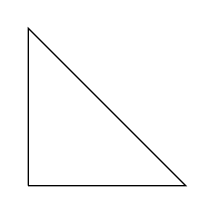
\begin{tikzpicture}
\draw (0,0) -- (0,2) -- (2,0)-- (0,0);
\end{tikzpicture}
\end{document}